\section{Structural Analysis}
\label{sec:structural-analysis}

Do the three graphs share common statistical signatures, or does each level have its own structural character? The answer bears directly on the central tension of this paper: universal patterns---such as heavy-tailed degree distributions or scale-free vulnerability---point to intrinsic features of mathematical dependency (product), while level-specific features---such as the bounded out-degree of proofs or the depth compression of the module graph---reveal cognitive and linguistic constraints imposed by the production process.

The preceding sections defined each graph and reported its basic statistics: node and edge counts, edge classifications, and containment measurements. We now apply five network-analytic tools---degree distribution (\S\ref{sec:sa-degree}), DAG depth (\S\ref{sec:dag-depth}), centrality (\S\ref{sec:sa-centrality}), community detection (\S\ref{sec:sa-community}), and robustness (\S\ref{sec:sa-robustness})---uniformly across all three graph levels. Organizing the analyses by method rather than by graph makes cross-level patterns immediately visible. We also include a declaration-level analysis that has no module or namespace counterpart: the theorem/lemma importance validation (\S\ref{sec:thm-vs-lemma}).

Unless stated otherwise, module-level statistics are reported for both the raw module graph $G_{\mathrm{module}}$ and its transitive reduction $G_{\mathrm{module}}^{-}$, to distinguish genuine logical necessity from cognitive redundancy (\S\ref{sec:transitive-reduction}).

%% ====================================================================
\subsection{Degree Distributions}
\label{sec:sa-degree}

The degree distribution is the most basic statistical fingerprint of a network. Its shape encodes information about the network's growth mechanism: a power-law tail suggests preferential attachment, where a small number of hubs continually attract new connections; a lognormal tail suggests multiplicative processes with many independent contributing factors; an exponential decay suggests uniform random connectivity. For our purposes, comparing degree distributions across the three graphs answers a pointed question: do human organization (module level) and mathematical logic (declaration level) produce the same distributional shape? Agreement would point to a shared generative mechanism; disagreement would implicate level-specific organizational forces.

We focus on three dimensions of comparison: (i)~the \emph{symmetry} between in-degree and out-degree---reflecting the directional structure of dependency; (ii)~\emph{tail behavior}---the severity of the heavy tail and the best-fitting distributional model; and (iii)~the \emph{effect of transitive reduction}---separating explicit human choices from logically necessary dependencies.

\subsubsection{Module Level}
\label{sec:degree-distribution}

In $G_{\mathrm{module}}$, the out-degree $\deg^{+}(m) = |\mathrm{imports}(m)|$: it counts the number of modules that $m$ directly imports. The in-degree $\deg^{-}(m)$ counts how many other modules depend on~$m$.
Structurally, in-degree measures how foundational a module is---how many others build upon it---while out-degree measures how much of the library a module assembles. A high in-degree module is \emph{infrastructure}; a high out-degree module is an \emph{integrator}.

\begin{table}[H]
\centering
\caption{Degree statistics for $G_{\mathrm{module}}$ and its transitive reduction~$G_{\mathrm{module}}^{-}$.}
\label{tab:degree-stats}
\begin{tabular}{lrrrr}
\toprule
& \multicolumn{2}{c}{$G_{\mathrm{module}}$} & \multicolumn{2}{c}{$G_{\mathrm{module}}^{-}$} \\
\cmidrule(lr){2-3} \cmidrule(lr){4-5}
& In-degree & Out-degree & In-degree & Out-degree \\
\midrule
Mean   & $3.12$ & $3.12$ & $2.57$ & $2.57$ \\
Median & $2$    & $3$    & $1$    & $2$    \\
Std    & $4.69$ & $4.12$ & $3.91$ & $1.83$ \\
Max    & $167$  & $315$  & $151$  & $70$   \\
\bottomrule
\end{tabular}
\end{table}

The module with the highest in-degree in both graphs is \module{Mathlib.Init} ($\deg^{-} = 167$ in $G_{\mathrm{module}}$, $151$ in $G_{\mathrm{module}}^{-}$), the foundational module that most files depend on. Other high in-degree modules include \module{Tactic.Common} ($74$), \module{Analysis.Normed.Group.Basic} ($57$), and \module{Algebra.Ring.Defs} ($42$). The highest out-degree belongs to \module{Mathlib.Tactic} ($315$ in $G_{\mathrm{module}}$), which serves as an umbrella file aggregating tactic imports; transitive reduction reduces this to~$60$.

We plot the degree distributions on log--log axes (Figure~\ref{fig:degree-distribution}).

\begin{figure}[H]
\centering
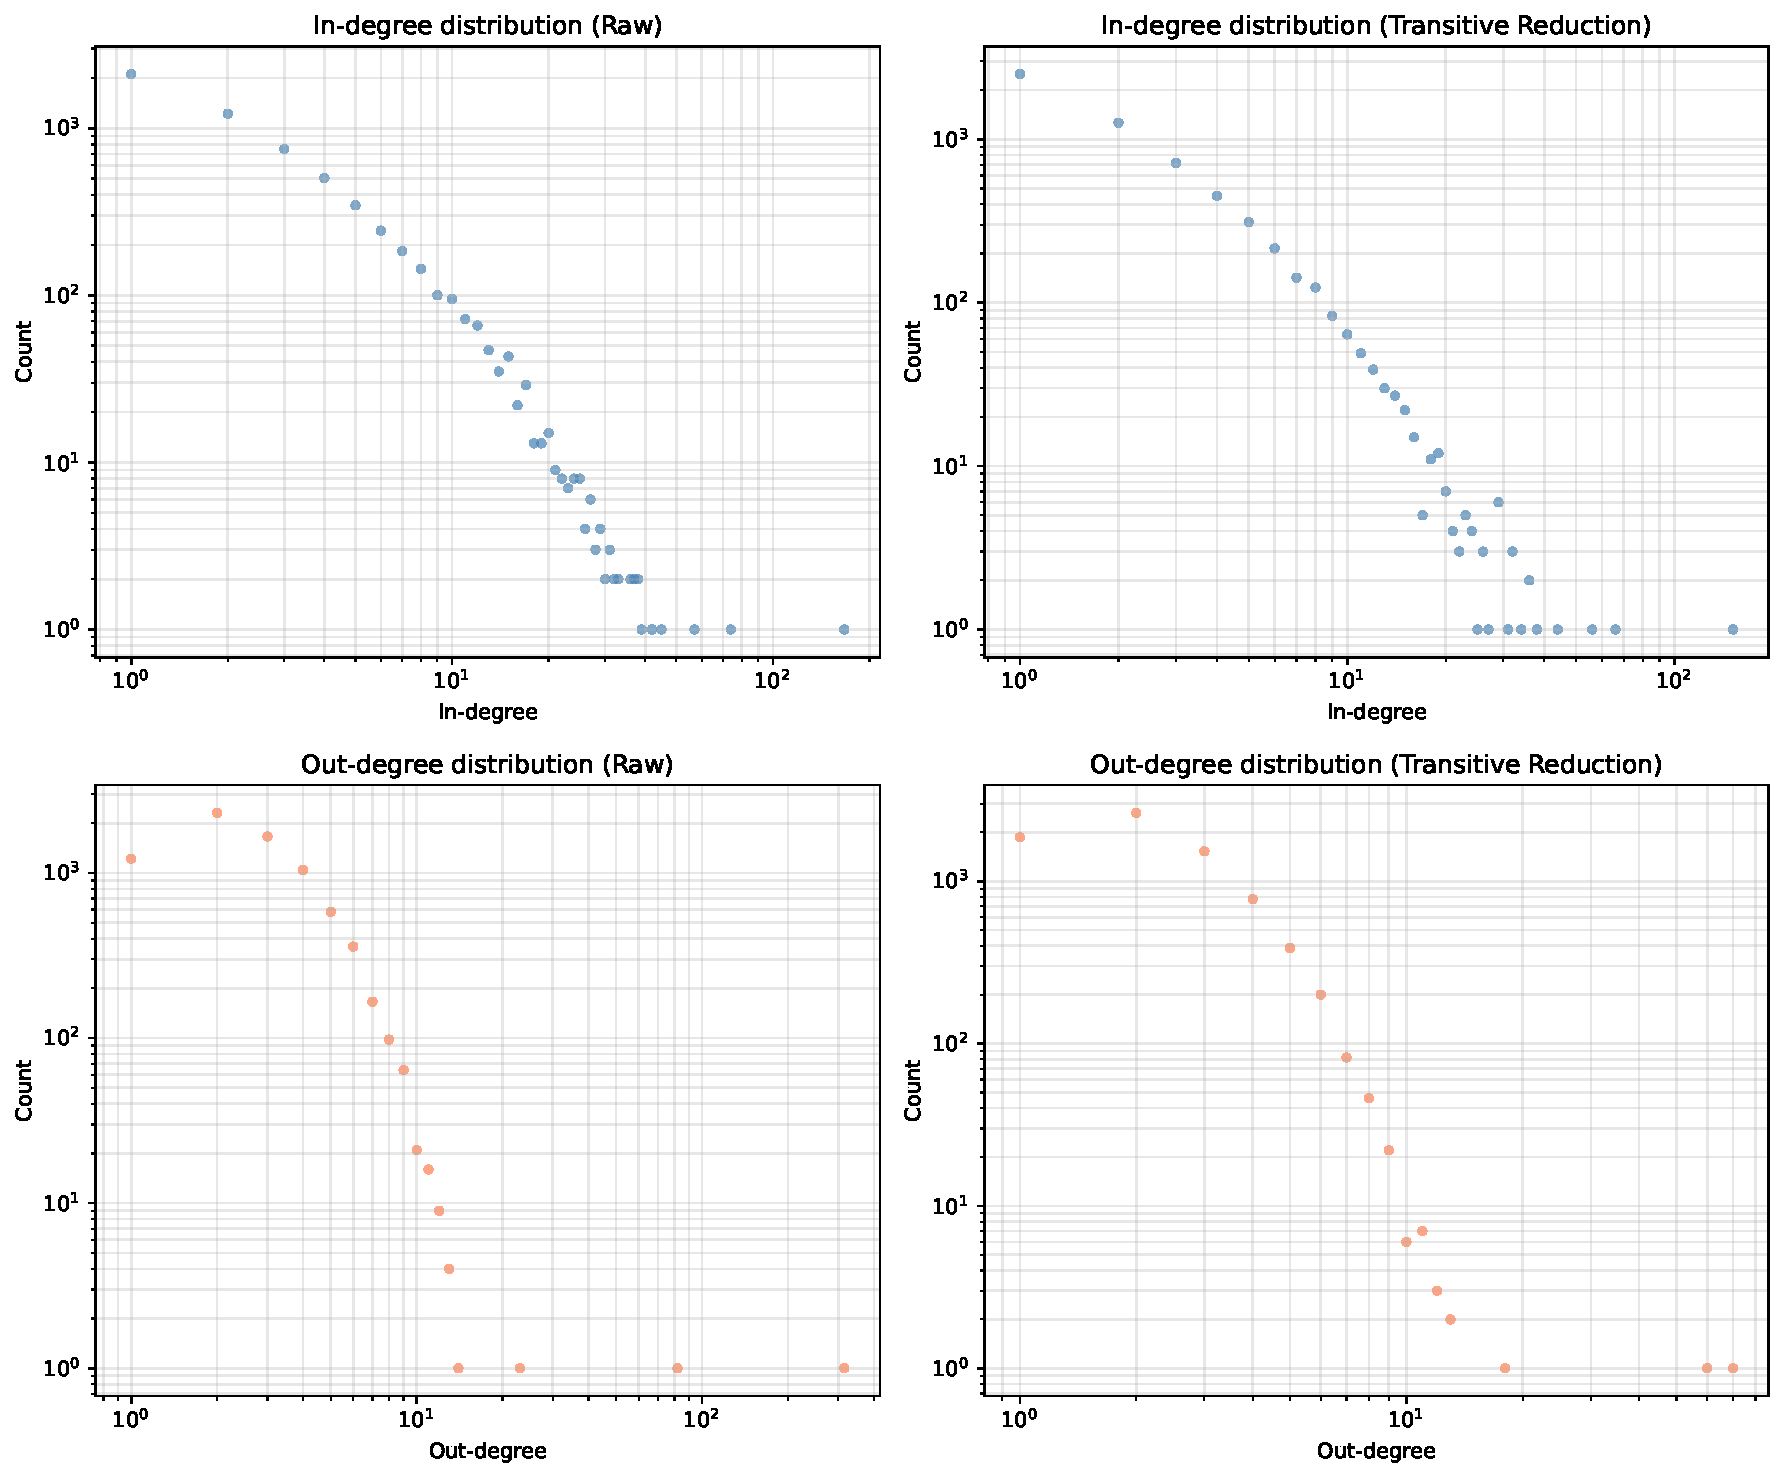
\includegraphics[width=\textwidth]{analysis/degree_distribution.pdf}
\caption{In-degree (blue) and out-degree (orange) distributions on log--log axes for $G_{\mathrm{module}}$ (left) and $G_{\mathrm{module}}^{-}$ (right). Dashed lines show power-law references $k^{-\gamma}$. Two features are visually salient: (i)~the in-degree distributions are nearly identical across the two panels, confirming that transitive reduction barely affects how many modules depend on a given file; (ii)~the out-degree tail contracts sharply under transitive reduction (maximum dropping from $315$ to $70$), reflecting the removal of redundant umbrella imports.}
\label{fig:degree-distribution}
\end{figure}

\begin{remark}
Both degree distributions are heavy-tailed but do not cleanly fit a power law. The out-degree distribution, in particular, becomes much more concentrated after transitive reduction (maximum dropping from $315$ to $70$, standard deviation from $4.12$ to $1.83$), indicating that many high-out-degree imports are transitively redundant.
In contrast, the in-degree distribution is barely affected by transitive reduction (maximum: $167 \to 151$; standard deviation: $4.69 \to 3.91$). This asymmetry has a structural explanation: redundant edges arise primarily from developers importing umbrella modules---an act that inflates the importer's out-degree without changing the importee's in-degree. The cognitive redundancy identified in \S\ref{sec:transitive-reduction} is \emph{directional}: it lives in the ``I depend on others'' direction, not the ``others depend on me'' direction.
This directional asymmetry connects to the tree $T$: developers inflate their out-degree by importing umbrella modules that aggregate entire sub-hierarchies---effectively borrowing $T$'s cognitive categories as navigational shortcuts. The redundancy is not random; it follows the contours of~$T$.
\end{remark}

\subsubsection{Declaration Level}
\label{sec:thm-degree}

The degree statistics of $G_{\mathrm{thm}}$ reveal a striking asymmetry between the two directions of dependency.

\begin{table}[ht]
\centering
\caption{Degree statistics for $G_{\mathrm{thm}}$.}
\label{tab:thm-degree}
\begin{tabular}{lrr}
\toprule
Statistic & In-degree & Out-degree \\
\midrule
Mean    & $27.38$    & $27.38$ \\
Median  & $1$        & $19$ \\
Std Dev & $620.10$   & $29.18$ \\
Max     & $89{,}936$ & $522$ \\
Zero-degree nodes & $119{,}633$ & $367$ \\
\bottomrule
\end{tabular}
\end{table}

The in-degree distribution has median~$1$ but mean~$27$ and standard deviation~$620$---a ratio of standard deviation to mean exceeding~$22$, indicating extreme concentration. A handful of declarations accumulate tens of thousands of citations while the majority are referenced at most once. The out-degree distribution, by contrast, has median~$19$, standard deviation~$29$, and maximum~$522$---a far more concentrated profile.

To test whether these distributions follow a power law, we apply the Clauset--Shalizi--Newman method (\S\ref{sec:prelim-powerlaw}).

\begin{table}[ht]
\centering
\caption{Power law fit and distribution comparisons for $G_{\mathrm{thm}}$. The likelihood ratio $R > 0$ favors power law; $R < 0$ favors the alternative. A $p$-value below $0.05$ indicates a statistically significant comparison.}
\label{tab:thm-powerlaw}
\begin{tabular}{lrrrr}
\toprule
& \multicolumn{2}{c}{In-degree} & \multicolumn{2}{c}{Out-degree} \\
\cmidrule(lr){2-3} \cmidrule(lr){4-5}
Metric & Value & $p$ & Value & $p$ \\
\midrule
$\alpha$ (exponent)     & $1.781$ & --- & $2.936$ & --- \\
$x_{\min}$              & $20$    & --- & $38$    & --- \\
$\sigma$ (std.\ error)  & $0.005$ & --- & $0.008$ & --- \\
Tail fraction           & $11.1\%$ & --- & $20.6\%$ & --- \\
\midrule
vs.\ Lognormal ($R$)          & $-2.48$   & $0.174$   & $-1{,}452.5$ & $\approx 0$ \\
vs.\ Exponential ($R$)        & $+28{,}766$ & $\approx 0$ & $-239.9$ & $0.014$ \\
vs.\ Stretched Exp.\ ($R$)    & $+105.8$  & $\approx 0$ & $-1{,}495.9$ & $\approx 0$ \\
vs.\ Truncated Power Law ($R$) & $-21.5$  & $\approx 0$ & $-1{,}509.5$ & $\approx 0$ \\
\bottomrule
\end{tabular}
\end{table}

For in-degree, the tail ($k \ge 20$, comprising $11.1\%$ of non-zero values) is well described by a heavy-tailed distribution with exponent $\alpha \approx 1.78$. Pure power law decisively beats exponential and stretched exponential alternatives, but a \emph{truncated power law} provides a significantly better fit ($R = -21.5$, $p \approx 0$), and the comparison with lognormal is inconclusive ($p = 0.17$). This pattern---heavy tail, uncertain between power law and lognormal, best fit by a truncated power law---is characteristic of many real-world networks~\cite{clauset2009}.

For out-degree, the picture is categorically different: \emph{every} alternative distribution significantly outperforms pure power law. The best fits are lognormal and truncated power law, both with overwhelmingly negative likelihood ratios.

\begin{remark}
\label{rem:thm-degree-asymmetry}
This asymmetry has a structural explanation that connects directly to the central tension of the paper. In-degree measures how often a declaration is \emph{cited}---a cumulative, open-ended quantity determined by the logical structure of the completed library (the product). There is no upper bound: \decl{OfNat.ofNat} can be cited by any proof that involves a numeral, and its in-degree ($89{,}936$) reflects a form of preferential attachment in which foundational declarations attract ever more dependents. Out-degree, by contrast, measures how many premises a single proof \emph{invokes}---a quantity bounded by the cognitive and logical complexity of that proof (the process). No human-written proof cites $90{,}000$ lemmas; the maximum out-degree of~$522$ reflects the practical ceiling of proof complexity. The in-degree distribution records the product; the out-degree distribution records the process.
\end{remark}

\begin{figure}[ht]
\centering
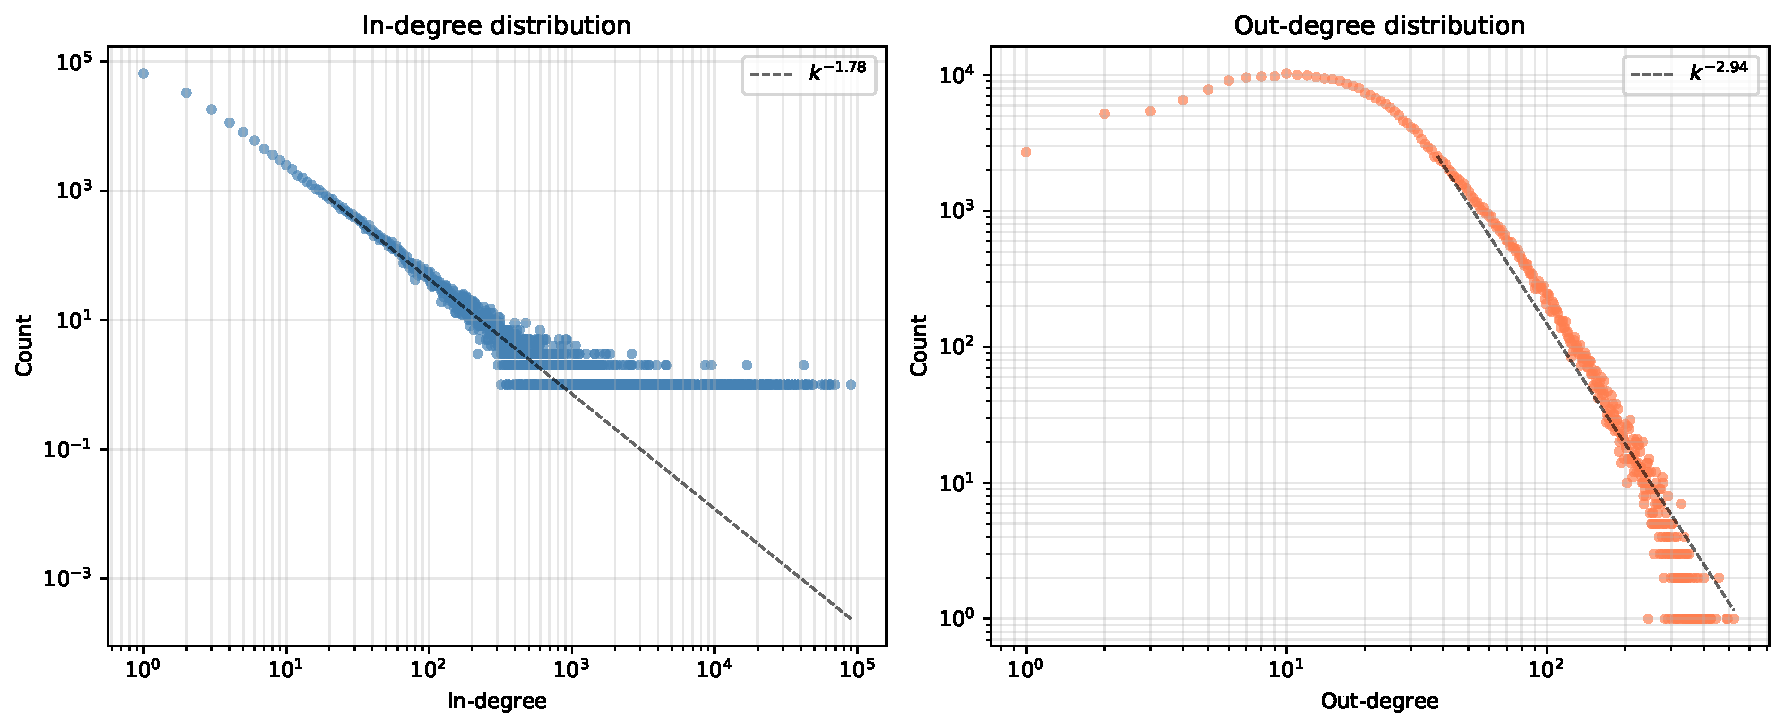
\includegraphics[width=\textwidth]{analysis/thm_degree_distribution.pdf}
\caption{Degree distributions of $G_{\mathrm{thm}}$ on log--log axes. Left: in-degree, with power law fit (gold line, $\alpha = 1.78$, $x_{\min} = 20$). Right: out-degree. The in-degree tail extends over four orders of magnitude; the out-degree distribution is sharply bounded.}
\label{fig:thm-degree}
\end{figure}

\begin{remark}[Transitive reduction at the theorem level]
\label{rem:thm-transitive-reduction}
In contrast to the module graph, where transitive reduction removes $17.5\%$ of edges (\S\ref{sec:transitive-reduction}), the theorem--premise graph does not admit a meaningful transitive reduction. In $G_{\mathrm{module}}$, redundant edges arise from deliberate human choices---developers importing umbrella modules for cognitive convenience. In $G_{\mathrm{thm}}$, every edge is extracted mechanically from the proof term by the kernel: if a premise appears in the proof, the edge exists, regardless of whether that premise could be reached indirectly through other premises. The distinction is significant: module-level redundancy measures the gap between what the compiler requires and what the human chooses; at the theorem level, this gap vanishes, because the data already records exactly what the compiler sees.
\end{remark}

\subsubsection{Namespace Level}
\label{sec:ns-degree}

We examine the degree distribution of $G_{\mathrm{ns}}^{(2)}$, the namespace graph at depth~$2$. We choose $k = 2$ because it occupies the sweet spot of the containment decay curve (Table~\ref{tab:containment-decay}): depth~$1$ is too coarse ($3{,}184$ namespaces, comparable to the top-level directory partition), while depth~$3$ and beyond add almost no new cross-boundary structure (containment saturates at ${\sim}13\%$). At depth~$2$, the $10{,}097$ namespaces correspond to familiar mathematical groupings---\ns{Nat.Prime}, \ns{CategoryTheory.Functor}, \ns{MeasureTheory.Measure}---and provide enough nodes for meaningful network analysis. The graph has $332{,}081$ edges (unique namespace pairs), carrying a total weight of $7{,}234{,}844$ declaration-level dependencies.

\begin{table}[ht]
\centering
\caption{Degree statistics for $G_{\mathrm{ns}}^{(2)}$ (unweighted).}
\label{tab:ns-degree-stats}
\begin{tabular}{lrr}
\toprule
& In-degree & Out-degree \\
\midrule
Mean        & $32.9$    & $32.9$ \\
Median      & $1$       & $14$ \\
Std         & $223.2$   & $59.3$ \\
Max         & $9{,}846$ & $3{,}075$ \\
Zero-degree & $3{,}920$ & $6$ \\
\bottomrule
\end{tabular}
\end{table}

The degree distribution is extremely skewed (Table~\ref{tab:ns-degree-stats}). The median in-degree of~$1$ versus a mean of~$33$ reveals a long tail: $3{,}920$ namespaces ($38.8\%$) have zero in-degree---they are referenced by no other namespace---while a handful attract thousands of incoming edges. The top namespaces by in-degree are \ns{\_root\_} ($9{,}846$), \ns{Eq} ($7{,}686$), \ns{OfNat} ($4{,}390$), \ns{Membership} ($3{,}407$), and \ns{Semiring} ($3{,}252$). By out-degree, the leaders are \ns{\_root\_} ($3{,}075$), \ns{MeasureTheory} ($687$), \ns{CategoryTheory} ($656$), and \ns{Polynomial} ($615$).

Power-law fitting (\S\ref{sec:prelim-powerlaw}) yields $\alpha = 1.60$ ($x_{\min} = 4$) for in-degree and $\alpha = 1.90$ ($x_{\min} = 13$) for out-degree. In both cases, a lognormal distribution provides a significantly better fit than a pure power law (likelihood ratio $R = -10.6$ and $R = -289.7$, respectively; $p < 0.01$). This mirrors the pattern observed for $G_{\mathrm{module}}$ (\S\ref{sec:degree-distribution}): heavy-tailed distributions that are not cleanly power-law.

\begin{figure}[ht]
\centering
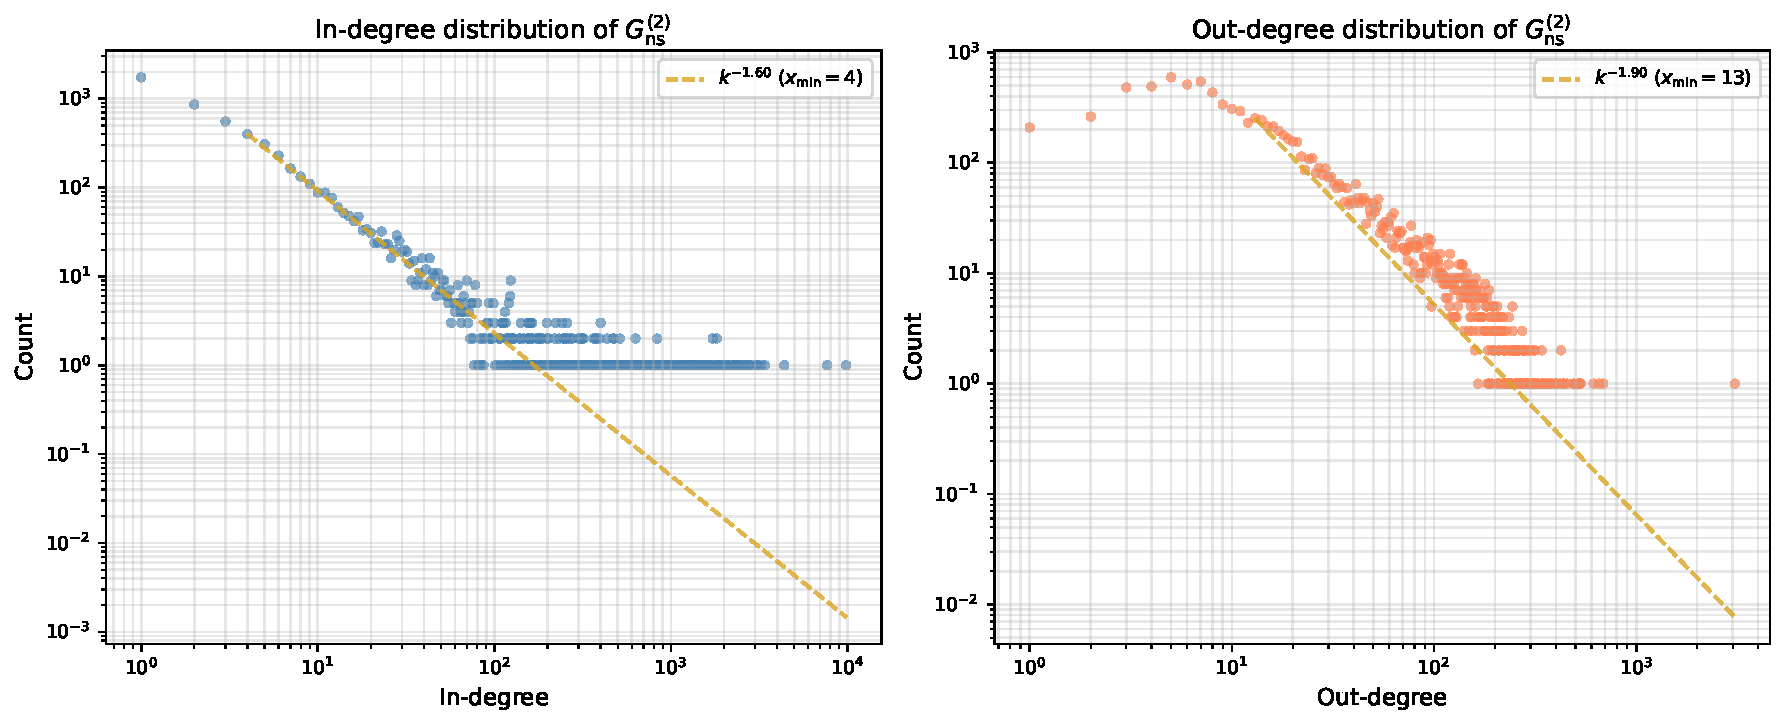
\includegraphics[width=\textwidth]{analysis/ns_degree_distribution.pdf}
\caption{Degree distributions of $G_{\mathrm{ns}}^{(2)}$ on log--log axes. Left: in-degree (\textcolor{blue!60!black}{blue}), with power-law reference (gold dashed, $\alpha = 1.60$, $x_{\min} = 4$). Right: out-degree (\textcolor{red!60!black}{coral}), with power-law reference ($\alpha = 1.90$, $x_{\min} = 13$). Both tails are heavy but better fit by a lognormal than a pure power law. The extreme outlier in the in-degree panel is \ns{\_root\_} ($\deg^{-} = 9{,}846$; see Remark~\ref{rem:root-artifact}).}
\label{fig:ns-degree}
\end{figure}

\begin{remark}[The \ns{\_root\_} artifact]
\label{rem:root-artifact}
The namespace \ns{\_root\_} dominates both in-degree and out-degree at depth~$2$. This is an artifact of the truncation rule in Definition~\ref{def:ns-graph}: declarations whose fully qualified names have fewer than three components---including foundational definitions such as \decl{Eq.refl}, \decl{Nat.succ}, and \decl{OfNat.ofNat}---are assigned to \ns{\_root\_}. This namespace is not a coherent conceptual domain; it is a catch-all for the shallow infrastructure of the Lean type system. Its extreme centrality reflects naming-depth convention rather than mathematical importance: the most foundational constructs carry the shortest names. In the analysis that follows, we note where \ns{\_root\_} distorts aggregate statistics.
\end{remark}

\paragraph{Cross-level comparison.}
All three levels share heavy-tailed degree distributions in which lognormal fits outperform pure power laws, confirming that the ``few hubs, many low-degree nodes'' pattern is a universal structural feature of the formalized library, independent of analysis granularity. But the differences are equally informative.

\emph{In-degree skewness intensifies with granularity.} At the module level, the in-degree distribution is moderately skewed (median~$2$, mean~$3.1$, max~$167$). At the declaration level, the skewness becomes extreme (median~$1$, mean~$27$, max~$89{,}936$): a handful of language-infrastructure declarations are cited by nearly every proof, while the majority are referenced at most once. The namespace level (median~$1$, mean~$33$, max~$9{,}846$) mirrors this pattern but is distorted by the \ns{\_root\_} artifact (Remark~\ref{rem:root-artifact}).

\emph{Out-degree reveals process constraints.} At the declaration level, out-degree is bounded by the cognitive and logical complexity of a single proof (mean~$27$, max~$522$)---a hard ceiling that no human-written proof exceeds. At the module level, out-degree reflects developer import choices; transitive reduction compresses the maximum from~$315$ to~$70$ and the standard deviation from~$4.12$ to~$1.83$, exposing the cognitive redundancy of umbrella imports (\S\ref{sec:transitive-reduction}). At the declaration level, by contrast, transitive reduction is not meaningful: every premise edge is mechanically extracted from the proof term (Remark~\ref{rem:thm-transitive-reduction}).

This pattern---shared distributional shape but divergent parameters and mechanisms---will recur in the centrality (\S\ref{sec:sa-centrality}) and community (\S\ref{sec:sa-community}) analyses that follow.

%% ====================================================================
\subsection{DAG Depth and Layered Structure}
\label{sec:dag-depth}

All sources (modules with no incoming edges) sit at level~$0$, while the unique sink \module{Tactic.Linter.DirectoryDependency} sits at level~$153$.

The depth of $G_{\mathrm{module}}$ is $153$, attained by a path from \module{NumberTheory.LSeries.PrimesInAP} (a leaf-level number theory result) down to \module{Tactic.Linter.DirectoryDependency} (a low-level linter utility). This path traverses number theory, special functions, measure theory, topology, order theory, logic, and tactic infrastructure---reflecting the deep dependency chain required to formalize analytic number theory.

$G_{\mathrm{module}}$ has $1{,}433$ source modules (files that no other \module{Mathlib} file imports) and exactly $1$~sink (\module{Tactic.Linter.DirectoryDependency}, the unique module with no imports within Mathlib). The topological levels partition $\mathcal{M}$ into $154$ layers, with a maximum layer width of $1{,}433$ (the source layer) and a median width of~$25$.

Notably, the layer-width profiles of $G_{\mathrm{module}}$ and $G_{\mathrm{module}}^{-}$ are nearly identical: the number of layers, the position of the peak, and the overall funnel shape are preserved under transitive reduction. This means that the vertical structure of the dependency chain reflects genuine logical necessity rather than cognitive redundancy---the 17.5\% redundant edges identified in \S\ref{sec:transitive-reduction} add lateral shortcuts within layers but do not alter the depth of the graph.

A secondary peak is visible near level~$126$, where approximately $59$ modules concentrate---roughly $6$ to $15$ times the width of surrounding layers. This anomaly warrants further investigation; it may reflect a layer of tactic infrastructure or a mathematical theory that branches into many parallel lemmas at a specific depth.

\begin{figure}[H]
\centering
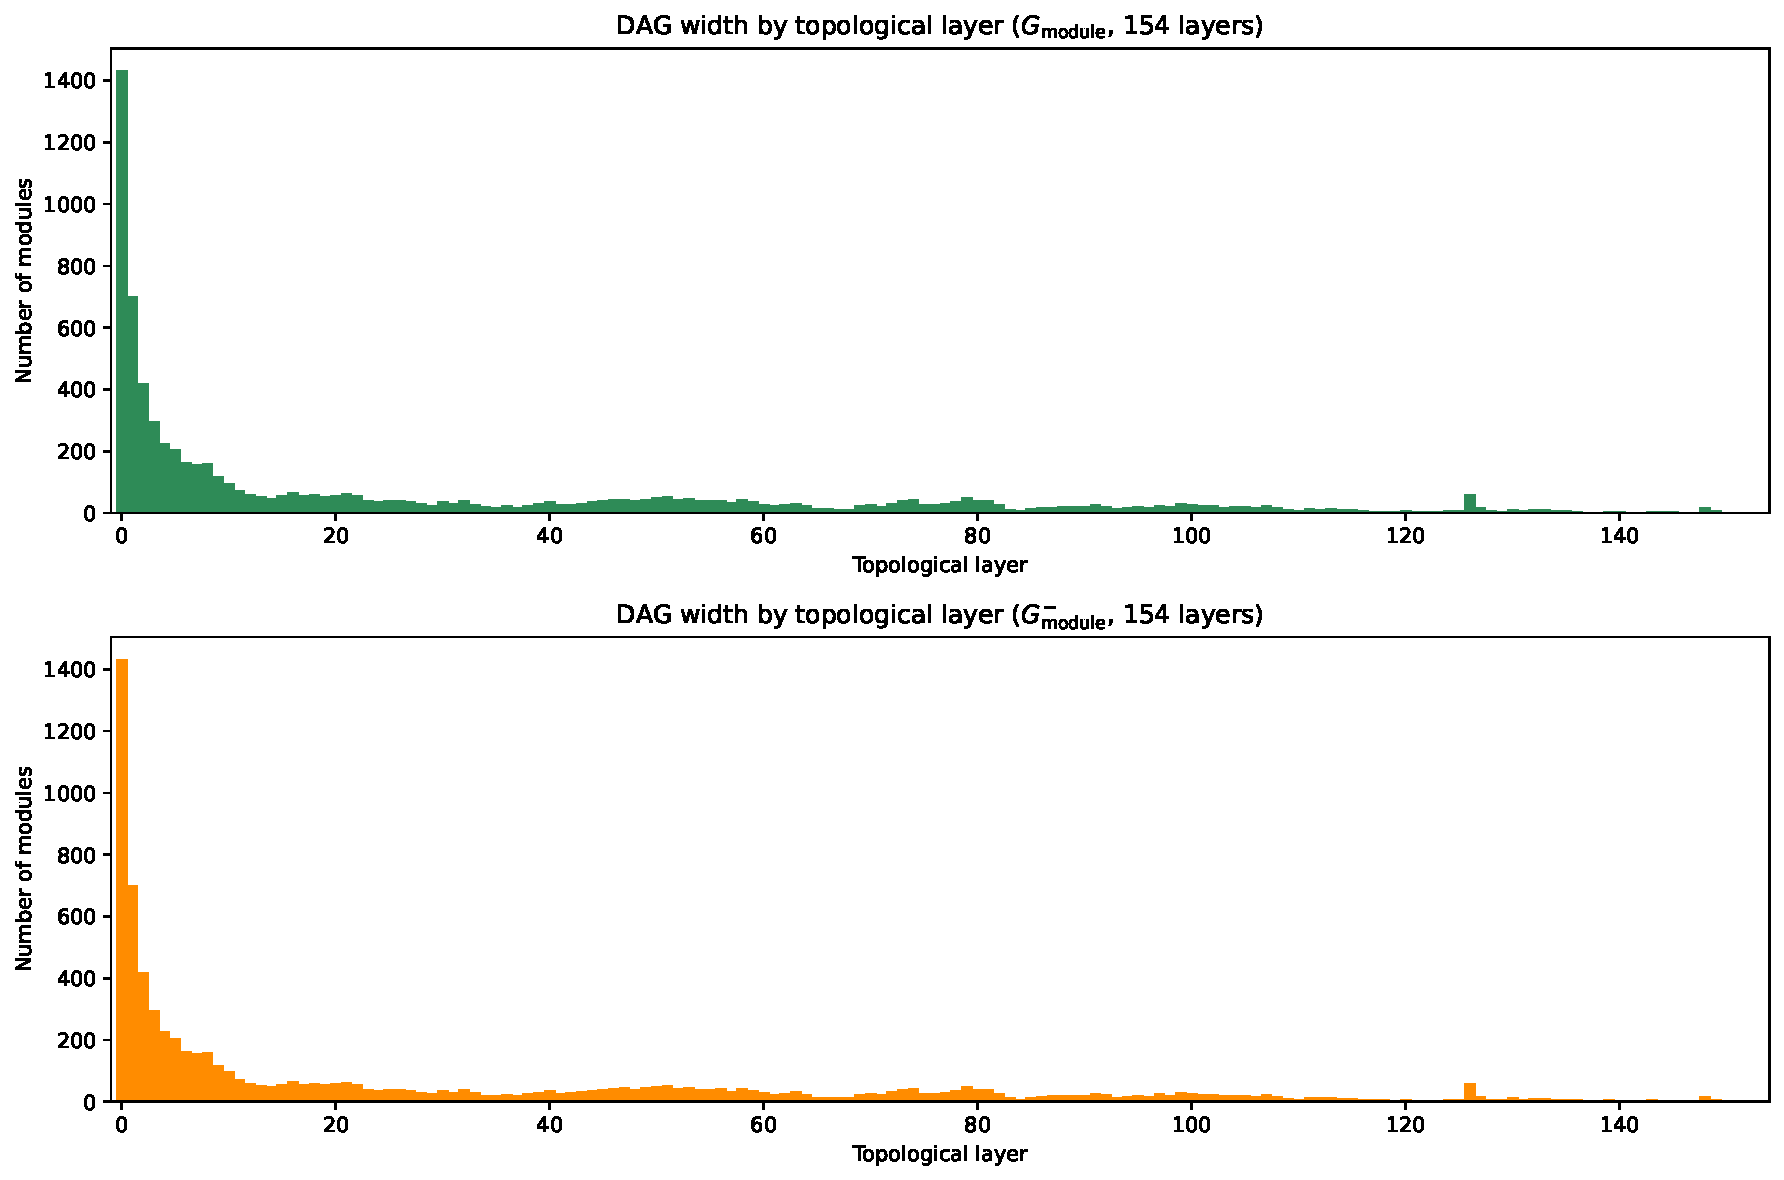
\includegraphics[width=\textwidth]{analysis/dag_structure.pdf}
\caption{DAG width by topological layer for $G_{\mathrm{module}}$ (top) and $G_{\mathrm{module}}^{-}$ (bottom). The distributions share a characteristic funnel shape: a sharp peak at level~$0$ (over $1{,}400$ leaf modules), a rapid decay through the first $20$ layers, a long tail extending to level~$153$, and a secondary peak near level~$126$. The near-identical profiles confirm that the funnel topology arises from logical necessity, not from redundant imports.}
\label{fig:dag-structure}
\end{figure}

\begin{remark}
The layer-width profile has a characteristic ``funnel'' shape: very wide at the top (many independent leaf files), narrowing through the middle layers (where mathematical theories converge), and tapering to a single sink at the bottom. This shape reflects the fact that advanced mathematics is built on a narrow foundation of shared definitions and tactics. This narrow waist also has engineering consequences: any change to a module in the bottleneck layers propagates upward through a large fraction of the library, creating recompilation cascades whose cost grows with the depth of the funnel.
\end{remark}

\begin{remark}[Module depth and import symmetry]
\label{rem:import-depth-symmetry}
The DAG depth of~$153$ layers describes the topological extent of the dependency chain. A different notion of depth---the \emph{module depth}, i.e., the number of dot-separated components of a module's fully qualified name---describes how deeply a module sits in the naming hierarchy~$T$. Module depth is concentrated: $55.7\%$ of modules have depth~$4$ (e.g., \module{Mathlib.Data.Nat.Basic}), with a mean of~$4.22$. Import edges exhibit near-perfect depth symmetry: $55.4\%$ connect modules at the same naming depth, $23.3\%$ point from deeper to shallower, and $21.3\%$ from shallower to deeper (mean difference~$+0.03$). Only~$1.3\%$ of imports target modules at depth~$\le 2$. Developers import \emph{laterally}---peer to peer within the same naming stratum---rather than vertically across naming layers. As we shall see in \S\ref{sec:cross_level}, this symmetry contrasts sharply with the declaration-level dependency graph, where $37.6\%$ of edges flow from deeper to shallower namespaces and the mean depth difference rises to~$+0.36$: the module graph compresses and hides the strong infrastructure pull that the declaration graph reveals.
\end{remark}

%% ====================================================================
\subsection{Centrality}
\label{sec:sa-centrality}

\subsubsection{Module Level}
\label{sec:centrality}

We compare three centrality measures---in-degree, PageRank, and betweenness (Definition~\ref{def:pagerank}--\ref{def:betweenness})---to identify the most structurally important modules.

\begin{table}[H]
\centering
\caption{Top~10 modules by in-degree, PageRank, and betweenness centrality in $G_{\mathrm{module}}$.}
\label{tab:centrality}
\small
\begin{tabular}{rlrlrl}
\toprule
\multicolumn{2}{c}{In-degree} & \multicolumn{2}{c}{PageRank} & \multicolumn{2}{c}{Betweenness} \\
\cmidrule(lr){1-2} \cmidrule(lr){3-4} \cmidrule(lr){5-6}
$\deg^{-}$ & Module & PR & Module & $c_B$ & Module \\
\midrule
167 & \module{Init}               & .0435 & \module{Init}              & .0113 & \module{Tactic.Common} \\
 74 & \module{Tactic.Common}      & .0316 & \module{Tactic.Linter.Header} & .0037 & \module{Init} \\
 57 & \module{AN.Group.Basic}     & .0285 & \module{Tactic.Linter.DD}  & .0032 & \module{LA.Span.Basic} \\
 45 & \module{Util.CompileInd.}   & .0058 & \module{Tactic.TypeStar}   & .0030 & \module{AN.Module.FD} \\
 42 & \module{Algebra.Ring.Defs}  & .0048 & \module{Algebra.Group.Defs} & .0024 & \module{Analysis.RCLike} \\
 39 & \module{ABO.Finset.Basic}   & .0038 & \module{Tactic.Basic}      & .0021 & \module{AS.Limits.Basic} \\
 38 & \module{Algebra.Field.Defs} & .0037 & \module{CT.Equivalence}    & .0020 & \module{AS.Limits.Normed} \\
 38 & \module{Algebra.Group.Basic}& .0033 & \module{Logic.Function}    & .0019 & \module{LA.Determinant} \\
 37 & \module{Tactic.Fin.Attr}    & .0030 & \module{Logic.Equiv.Defs}  & .0019 & \module{CT.Category.Basic} \\
 37 & \module{Tactic.TypeStar}    & .0030 & \module{CT.Opposites}      & .0017 & \module{Tactic.NormNum} \\
\bottomrule
\end{tabular}
\end{table}

\noindent
\textit{Abbreviations:} AN = \module{Analysis.Normed}, LA = \module{LinearAlgebra}, CT = \module{CategoryTheory},\\
ABO = \module{Algebra.BigOperators.Group}, AS = \module{Analysis.SpecificLimits},\\
FD = \module{FiniteDimension}, DD = \module{DirectoryDependency}, CompileInd.\ = \module{CompileInductive}, Fin.\ = \module{Finiteness}.

We compare in-degree, PageRank, and betweenness pairwise in Figure~\ref{fig:centrality}. Out-degree is omitted from this comparison because it measures a module's role as an \emph{importer}---how many prerequisites it gathers---rather than its structural position within the network. Moreover, as shown in \S\ref{sec:degree-distribution}, high out-degree values largely reflect redundant umbrella imports and collapse under transitive reduction, making out-degree a poor proxy for structural importance.

\begin{figure}[H]
\centering
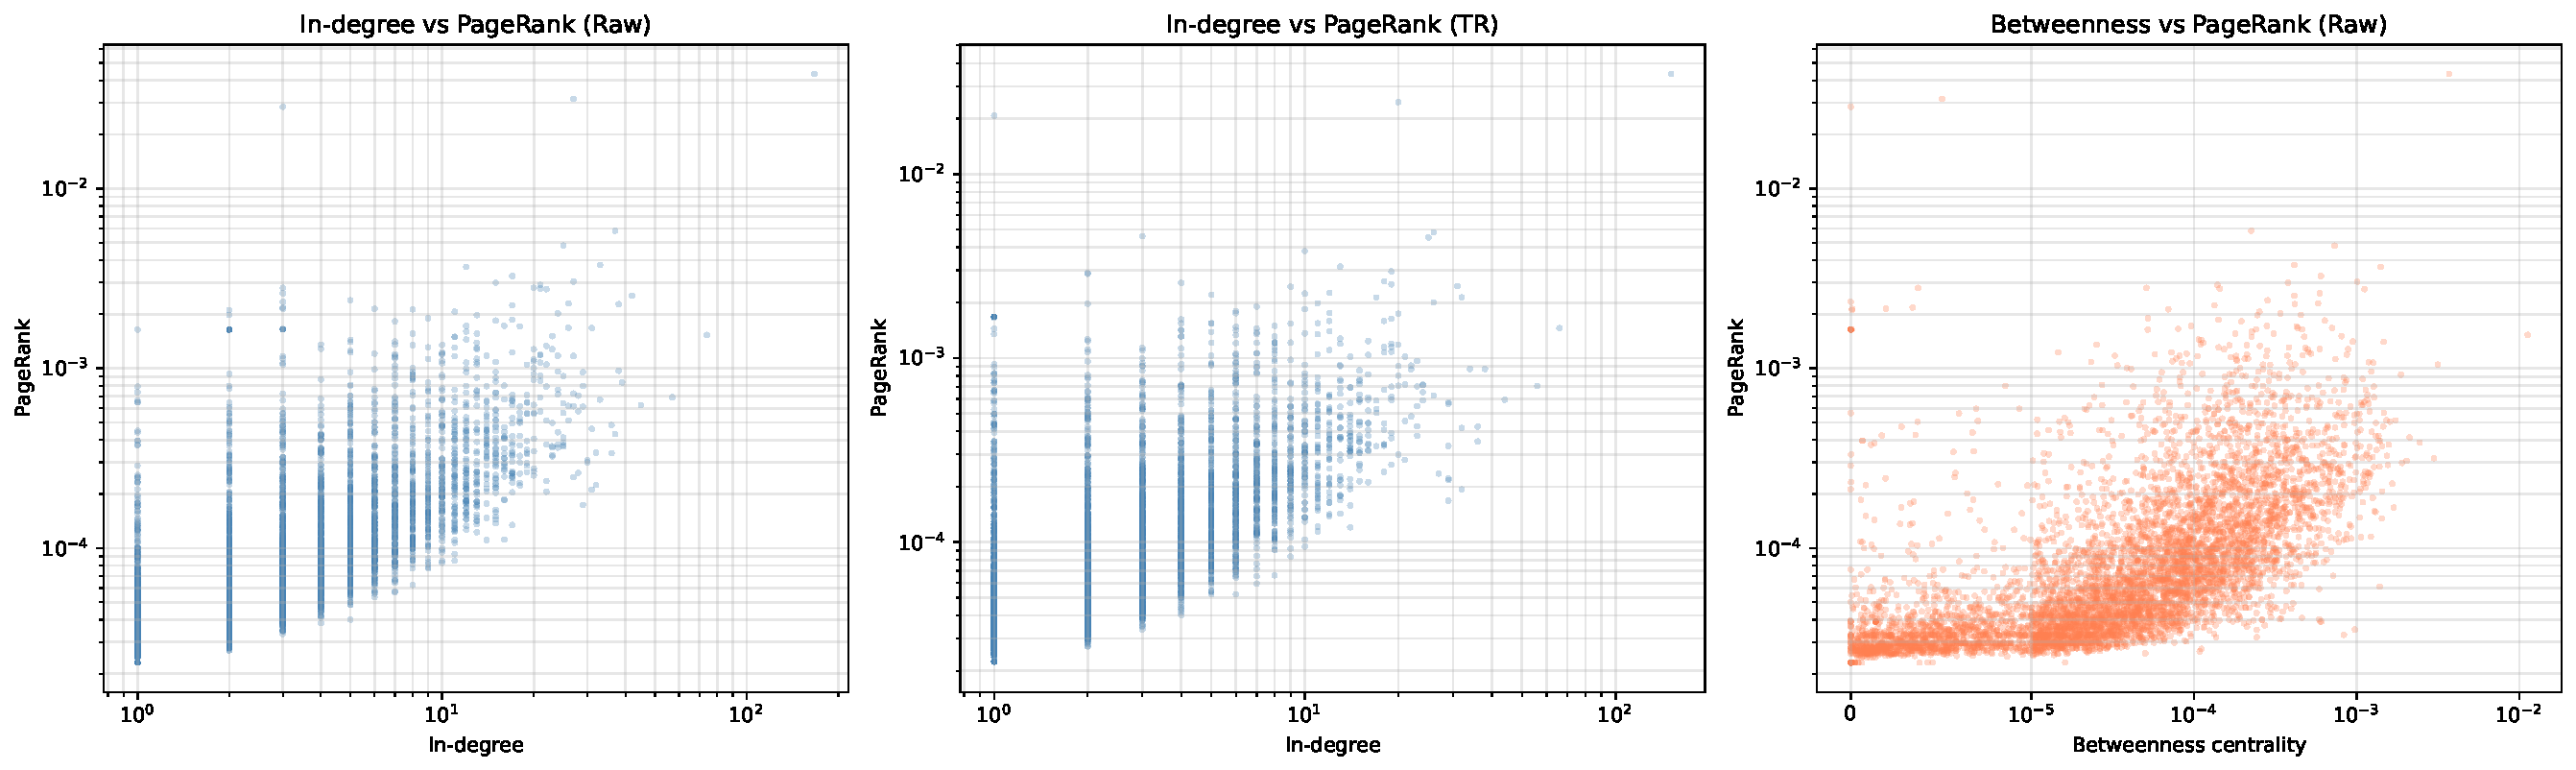
\includegraphics[width=\textwidth]{analysis/centrality_analysis.pdf}
\caption{Scatter plots of centrality measures in $G_{\mathrm{module}}$; each point represents one module. Left and center: in-degree vs.\ PageRank (raw and TR). Right: betweenness vs.\ PageRank (raw). If any two measures were equivalent, points would cluster along a diagonal line; the wide scatter in each panel confirms that the three centrality measures capture distinct structural roles. Notable outliers are labeled.}
\label{fig:centrality}
\end{figure}

The three rankings largely differ: the only module appearing in all three top-20 lists is \module{Mathlib.Init}. This divergence is not a technical detail---it is one of our central findings. It demonstrates that \emph{importance} in a formal mathematical library is irreducibly multidimensional: a module can be heavily used (high in-degree) without being foundational (high PageRank), and foundational without being a bridge (high betweenness). No single centrality measure captures the full structural role of a module; the three measures together define a taxonomy that we develop further in \S\ref{sec:module_conclusion}.

In particular, high-betweenness modules acquire their bridging role precisely by connecting regions of $G_{\mathrm{module}}$ that the tree $T$ separates. The top betweenness modules in Table~\ref{tab:centrality} typically sit at the boundary between top-level directories: they are the points where the logical structure of mathematics forces a passage across $T$'s cognitive borders.

In-degree identifies the most frequently \emph{imported} modules (foundational definitions and commonly used tactics). PageRank, which propagates importance along dependency chains, promotes modules deep in the import hierarchy such as \module{Tactic.Linter.Header} and low-level logic utilities. Betweenness centrality highlights \emph{bottleneck} modules through which many shortest paths pass, favoring files like \module{LinearAlgebra.Span.Basic} and \module{Analysis.Normed.Module.FiniteDimension} that bridge otherwise distant parts of the library.

\subsubsection{Declaration Level}
\label{sec:thm-centrality}

In \S\ref{sec:centrality}, we found that in-degree, PageRank, and betweenness centrality identify different structural roles at the module level. We now compute the same three measures on $G_{\mathrm{thm}}$ and find that the divergence between them is, if anything, more extreme.

\begin{table}[ht]
\centering
\caption{Top~10 declarations by in-degree, PageRank ($\alpha = 0.85$), and betweenness centrality (sampled, $k = 500$) in $G_{\mathrm{thm}}$.}
\label{tab:thm-centrality}
\small
\begin{tabular}{rlrlrl}
\toprule
\multicolumn{2}{c}{In-degree} & \multicolumn{2}{c}{PageRank} & \multicolumn{2}{c}{Betweenness} \\
\cmidrule(lr){1-2} \cmidrule(lr){3-4} \cmidrule(lr){5-6}
$\deg^{-}$ & Declaration & PR & Declaration & $c_B$ & Declaration \\
\midrule
$89{,}936$ & \decl{OfNat.ofNat}       & $.0151$ & \decl{CT.Category.mk}    & $.000338$ & \decl{Real} \\
$69{,}580$ & \decl{Eq.refl}           & $.0145$ & \decl{OfNat.mk}           & $.000338$ & \decl{Real.ofCauchy} \\
$65{,}437$ & \decl{DFunLike.coe}      & $.0140$ & \decl{outParam}           & $.000289$ & \decl{Rat.linearOrder} \\
$63{,}530$ & \decl{Membership.mem}    & $.0125$ & \decl{OfNat}              & $.000256$ & \decl{Real.pi} \\
$62{,}942$ & \decl{Eq.mpr}            & $.0123$ & \decl{CT.Category}        & $.000253$ & \decl{Real.$\exists$cos\_eq\_0} \\
$59{,}997$ & \decl{Set}               & $.0106$ & \decl{Eq.refl}            & $.000183$ & \decl{Rat.instIsStrictOrd.} \\
$58{,}686$ & \decl{Eq.trans}          & $.0097$ & \decl{Quiver}             & $.000177$ & \decl{Rat.le\_refl} \\
$56{,}019$ & \decl{Semiring.toNAR}    & $.0095$ & \decl{Quiver.mk}          & $.000164$ & \decl{Real.zero\_lt\_one} \\
$48{,}801$ & \decl{of\_eq\_true}      & $.0084$ & \decl{LE}                 & $.000157$ & \decl{Complex.log} \\
$48{,}295$ & \decl{PO.toPreorder}     & $.0084$ & \decl{LE.mk}              & $.000155$ & \decl{instSemiringNNReal} \\
\bottomrule
\end{tabular}
\end{table}

\noindent
\textit{Abbreviations:} CT = CategoryTheory, NAR = NonAssocSemiring, PO = PartialOrder, instIsStrictOrd.\ = instIsStrictOrderedRing, $\exists$cos\_eq\_0 = exists\_cos\_eq\_zero.

\medskip

The three columns of Table~\ref{tab:thm-centrality} have almost no overlap, and each tells a different story about the structure of \module{Mathlib}.

\emph{In-degree} is dominated by language infrastructure. The top entries---\decl{OfNat.ofNat}, \decl{Eq.refl}, \decl{DFunLike.coe}, \decl{Membership.mem}, \decl{Eq.mpr}---are type-class coercions and equality constructors that the elaborator inserts into virtually every proof term. Their prominence reflects the design of Lean~4, not the structure of mathematics. This contrasts with the module-level in-degree ranking (Table~\ref{tab:centrality}), where the top entry (\module{Mathlib.Init}) is a file that every module must import; the underlying mechanism---implicit foundational dependency---is analogous, but the theorem level reveals the specific \emph{declarations} responsible.

\emph{PageRank} promotes a different set of nodes: the constructors and types of category theory (\decl{CategoryTheory.Category.mk}, \decl{Quiver}, \decl{Quiver.mk}) and core algebraic infrastructure (\decl{OfNat}, \decl{LE}, \decl{Zero}). The key divergence from in-degree is \decl{CategoryTheory.Category.mk}: it ranks first in PageRank but does not appear in the in-degree top~$20$. Its PageRank reflects not its direct citation count but the fact that the entire $59{,}724$-node category theory subgraph depends on it transitively. PageRank captures \emph{recursive} importance---it identifies the foundations on which large, internally coherent subgraphs rest.

\emph{Betweenness centrality} reveals a third, entirely disjoint set of structurally critical declarations. The top entries---\decl{Real}, \decl{Real.ofCauchy}, \decl{Rat.linearOrder}, \decl{Real.pi}, \decl{Real.exists\_cos\_eq\_zero}---trace the construction chain of the real numbers. These nodes sit at the narrow passage connecting the algebraic world (rational numbers, ordered rings, number fields) to the analytic world (measure theory, complex analysis, probability). \decl{Real.pi} occupies rank~$4$ because $\pi$'s definition threads through number theory, trigonometry, and analysis, making it a crossroads of multiple mathematical disciplines. Only $34{,}564$ of $308{,}129$ nodes ($11.2\%$) have nonzero betweenness, confirming that shortest paths through $G_{\mathrm{thm}}$ are concentrated through a small number of critical bridges.

\begin{remark}
\label{rem:thm-centrality-vs-module}
The three-way divergence of centrality measures observed at the module level (\S\ref{sec:centrality}) intensifies at the theorem level: no declaration appears in all three top-$10$ lists of Table~\ref{tab:thm-centrality}. The taxonomy of importance proposed in \S\ref{sec:module_conclusion}---\emph{vocabulary} (in-degree), \emph{axiomatic core} (PageRank), \emph{structural bridges} (betweenness)---receives sharper instantiation here. At the module level, the centrality rankings are partially confounded by file-organization artifacts (e.g., \module{Mathlib.Init} ranks high in all three measures simply because it is imported by every file). At the theorem level, these artifacts are stripped away, and the three measures separate cleanly into language infrastructure (in-degree), mathematical foundations (PageRank), and inter-disciplinary bridges (betweenness).
\end{remark}

\subsubsection{Namespace Level}
\label{sec:ns-centrality}

As in \S\ref{sec:centrality} and \S\ref{sec:thm-centrality}, we compute PageRank and betweenness centrality (Definition~\ref{def:pagerank}--\ref{def:betweenness}; $\alpha = 0.85$, weighted; $k = 300$ samples) to identify structurally important namespaces.

\begin{table}[ht]
\centering
\caption{Top~10 namespaces by PageRank and betweenness centrality in $G_{\mathrm{ns}}^{(2)}$.}
\label{tab:ns-centrality}
\small
\begin{tabular}{rlrl}
\toprule
\multicolumn{2}{c}{PageRank} & \multicolumn{2}{c}{Betweenness} \\
\cmidrule(lr){1-2} \cmidrule(lr){3-4}
PR & Namespace & $c_B$ & Namespace \\
\midrule
.247 & \ns{\_root\_}          & .248 & \ns{\_root\_} \\
.035 & \ns{Eq}                & .065 & \ns{And} \\
.017 & \ns{Set}               & .043 & \ns{Eq} \\
.015 & \ns{Iff}               & .036 & \ns{Exists} \\
.014 & \ns{OfNat}             & .031 & \ns{Function} \\
.012 & \ns{Real}              & .030 & \ns{Nat} \\
.012 & \ns{Nat}               & .029 & \ns{CategoryTheory} \\
.012 & \ns{CategoryTheory}    & .019 & \ns{MeasureTheory} \\
.010 & \ns{Preorder}          & .018 & \ns{Set} \\
.008 & \ns{Semiring}          & .017 & \ns{Module} \\
\bottomrule
\end{tabular}
\end{table}

Excluding the \ns{\_root\_} artifact (Remark~\ref{rem:root-artifact}), the two rankings reveal a clear separation (Table~\ref{tab:ns-centrality}). PageRank is dominated by mathematical infrastructure: \ns{Eq}, \ns{Set}, \ns{OfNat}, \ns{Real}, and \ns{Preorder}---the foundational types and structures on which proofs ultimately rest. Betweenness centrality, by contrast, promotes logical connectives and bridging concepts: \ns{And}, \ns{Exists}, and \ns{Function} occupy positions~$2$--$5$ by betweenness but do not appear in the PageRank top~$10$. These namespaces serve as structural bridges: proofs in distant mathematical theories must pass through logical connectives to compose their arguments.

This separation echoes the module-level finding of \S\ref{sec:centrality}, where no single module dominates all three centrality measures, and the declaration-level finding of \S\ref{sec:thm-centrality}, where in-degree, PageRank, and betweenness identify disjoint categories of importance. At the namespace level, the two available measures already diverge sharply, confirming that the multidimensionality of structural importance persists across all three granularities.

%% ====================================================================
\subsection{Community Structure}
\label{sec:sa-community}

\subsubsection{Declaration Level}
\label{sec:thm-community}

We apply Louvain community detection (\S\ref{sec:prelim-community}) to the largest weakly connected component of $G_{\mathrm{thm}}$ (converted to an undirected graph, $308{,}054$ nodes, $8{,}431{,}648$ undirected edges).

\begin{table}[ht]
\centering
\caption{Community detection summary for $G_{\mathrm{thm}}$.}
\label{tab:thm-community-summary}
\begin{tabular}{lr}
\toprule
Metric & Value \\
\midrule
Number of communities & $22$ \\
Modularity & $0.4757$ \\
Communities with ${>}1{,}000$ nodes & $7$ \\
Communities with ${>}100$ nodes & $11$ \\
\bottomrule
\end{tabular}
\end{table}

The modularity of $0.48$ indicates a moderately strong community structure---significantly above random ($0$) but below perfectly modular ($1$). If logical dependency alone determined community structure (pure product), modularity would be higher; if cognitive organization were independent of logic (pure process), it would approach zero. The intermediate value quantifies the partial---but incomplete---alignment between mathematical necessity and human practice. The $22$ communities are highly unequal: seven communities of more than $1{,}000$ nodes account for $99.1\%$ of the graph; the remaining fifteen communities contain fewer than $700$ nodes each.

\begin{table}[ht]
\centering
\caption{The seven major communities of $G_{\mathrm{thm}}$ (Louvain, $> 1{,}000$ nodes), with size, dominant mathematical theme, and top representatives by PageRank.}
\label{tab:thm-communities}
\small
\begin{tabular}{rrllp{4cm}}
\toprule
ID & Size & Theme & Top namespace(s) & Representatives \\
\midrule
0  & $63{,}763$ & Order / Sets / Filters & \ns{Set}, \ns{Filter}, \ns{Matroid} & \decl{LE}, \decl{Set}, \decl{Iff.intro}, \decl{Zero} \\
5  & $59{,}724$ & Category Theory & \ns{CategoryTheory} (69\%) & \decl{CT.Category.mk}, \decl{Quiver}, \decl{CT.CategoryStruct} \\
2  & $54{,}649$ & Algebra & \ns{LinearMap}, \ns{Matrix}, \ns{Module} & \decl{outParam}, \decl{Zero.mk}, \decl{Semiring} \\
1  & $49{,}739$ & Combinatorics / Discrete & \ns{List}, \ns{Finset}, \ns{SimpleGraph} & \decl{OfNat.mk}, \decl{Eq.refl}, \decl{List.nil} \\
11 & $38{,}245$ & Number Theory / Polynomials & \ns{Nat}, \ns{Int}, \ns{Polynomial} & \decl{OfNat}, \decl{Mul}, \decl{Semiring.mk} \\
7  & $37{,}368$ & Analysis / Probability & \ns{MeasureTheory}, \ns{Real} & \decl{Real}, \decl{MeasurableSpace} \\
8  & $2{,}773$ & Model Theory / Set Theory & \ns{FirstOrder}, \ns{SetTheory} & \decl{FirstOrder.Language.mk} \\
\bottomrule
\end{tabular}
\end{table}

These seven communities map recognizably onto traditional mathematical subdisciplines. The alignment is not imposed by the analysis; it emerges from the dependency topology alone. Louvain knows nothing about mathematical content---it optimizes modularity on the undirected edge structure---yet it recovers divisions (algebra vs.\ analysis, category theory vs.\ combinatorics) that correspond to centuries-old disciplinary boundaries.

To quantify the alignment between community structure and the namespace hierarchy, we compute the Normalized Mutual Information (NMI) and Adjusted Rand Index (ARI, Definition~\ref{def:nmi}--\ref{def:ari}) between two labelings of the $308{,}054$ nodes: the Louvain community assignment and the top-level namespace extracted from each declaration's module path.

\begin{table}[ht]
\centering
\caption{Alignment between Louvain communities and top-level namespaces.}
\label{tab:thm-nmi}
\begin{tabular}{lrl}
\toprule
Metric & Value & Interpretation \\
\midrule
NMI & $0.3432$ & Moderate association \\
ARI & $0.1817$ & Weak-to-moderate agreement \\
\bottomrule
\end{tabular}
\end{table}

The moderate NMI and low ARI confirm that dependency topology and namespace organization are \emph{related but far from identical}. The most striking case is \ns{CategoryTheory}: $97.4\%$ of its $42{,}094$ declarations fall into Community~$5$, and conversely, $68.7\%$ of Community~$5$ belongs to the \ns{CategoryTheory} namespace. This near-perfect correspondence is unique among the major communities. By contrast, the largest community (Community~$0$, $63{,}763$ nodes) draws its largest namespace contribution from root-level declarations ($17.1\%$), followed by \ns{Set} ($8.1\%$) and \ns{MeasureTheory} ($4.6\%$)---no single namespace dominates.

\begin{remark}
\label{rem:nmi-tension}
The NMI of $0.34$ provides a theorem-level metric for the tension between the module tree $T$ and the logical dependency graph $G$, extending the cross-namespace analysis of \S\ref{sec:cross-namespace}. At the module level, $37.1\%$ of reduced import edges cross namespace boundaries; at the theorem level, the NMI of $0.34$ quantifies the same phenomenon from a complementary angle---the dependency-based community structure aligns only moderately with the human-imposed namespace hierarchy. These two measures converge on the same conclusion: cognitive classification and logical structure are correlated but distinct, and the gap between them widens as granularity increases.

The exceptional case of category theory deserves emphasis. Its near-complete community--namespace alignment ($97.4\%$) suggests that category theory is not merely a namespace convention but a genuinely \emph{autonomous} mathematical discipline within \module{Mathlib}---its internal dependency structure is dense enough to form a self-contained community with minimal need for external foundations beyond the shared core. No other major namespace achieves this degree of self-containment.
\end{remark}

\subsubsection{Namespace Level}
\label{sec:ns-community}

Louvain community detection (\S\ref{sec:prelim-community}) on the undirected, weighted projection of $G_{\mathrm{ns}}^{(2)}$ yields $10$ communities with modularity $Q = 0.283$.

\begin{table}[ht]
\centering
\caption{Top five communities in $G_{\mathrm{ns}}^{(2)}$ by size, with representative namespaces (highest weighted in-degree within each community).}
\label{tab:ns-communities}
\begin{tabular}{rrl}
\toprule
ID & Size & Representative namespaces \\
\midrule
3 & $5{,}096$ & \ns{\_root\_}, \ns{Set}, \ns{Nat} \\
5 & $2{,}227$ & \ns{Semiring}, \ns{NonUnitalNonAssocSemiring}, \ns{DFunLike} \\
4 & $1{,}363$ & \ns{Eq}, \ns{CategoryTheory}, \ns{CategoryTheory.Functor} \\
0 & $1{,}041$ & \ns{Real}, \ns{Zero}, \ns{Field} \\
1 & $360$     & \ns{DivInvMonoid}, \ns{MulOne}, \ns{MulOneClass} \\
\bottomrule
\end{tabular}
\end{table}

The namespace-level community structure differs markedly from the declaration-level structure (\S\ref{sec:thm-community}). At the declaration level, Louvain detection produces $22$ communities with modularity $0.48$ and NMI~$= 0.34$ against the top-level namespace hierarchy. At the namespace level, the number of communities is smaller ($10$ vs.\ $22$), the modularity is lower ($0.283$ vs.\ $0.48$), and the NMI with the top-level directory falls to~$0.253$ (Table~\ref{tab:ns-communities}).

The lower modularity reflects the coarsening inherent in namespace aggregation. When thousands of declarations are collapsed into a single namespace node, the fine-grained community boundaries that Louvain detects at the declaration level are blurred. Edges between namespaces are weighted sums of many declaration-level edges, and the averaging effect smooths out the modular structure that exists at finer granularity. The largest community (ID~$3$, $5{,}096$ nodes) spans half the graph and lacks a coherent mathematical identity: its dominant members (\ns{\_root\_}, \ns{Set}, \ns{Nat}) are foundational constructs used across all disciplines. This contrasts with the declaration-level communities, where the largest communities map onto recognizable mathematical disciplines (\S\ref{sec:thm-community}).

%% ====================================================================
\subsection{Robustness}
\label{sec:sa-robustness}

\subsubsection{Module Level}
\label{sec:robustness}

$G_{\mathrm{module}}$ is weakly connected: all $7{,}563$ modules belong to a single weakly connected component. We assess robustness by measuring the impact of targeted node removal.

\begin{table}[H]
\centering
\caption{Effect of removing the top-5 modules (by in-degree or betweenness) on the number of weakly connected components.}
\label{tab:robustness}
\begin{tabular}{lrr}
\toprule
Removal strategy & \multicolumn{1}{c}{$G_{\mathrm{module}}$} & \multicolumn{1}{c}{$G_{\mathrm{module}}^{-}$} \\
\midrule
None (baseline)          & $1$  & $1$  \\
Top-5 by in-degree       & $29$ & $56$ \\
Top-5 by betweenness     & $20$ & $48$ \\
\bottomrule
\end{tabular}
\end{table}

Removing the five highest in-degree modules (\module{Init}, \module{Tactic.Common}, \module{Analysis.Normed.Group.Basic}, \module{Util.CompileInductive}, and \module{Algebra.Ring.Defs}) fragments the raw graph into $29$ components, though the largest component still contains $7{,}530$ of the original $7{,}563$ nodes. The effect is more pronounced on $G_{\mathrm{module}}^{-}$ ($56$ components), since transitive reduction removes the alternative paths that would otherwise keep the graph connected.

\begin{remark}
\label{rem:robustness}
The fragmentation is modest: even after targeted removal, over $99\%$ of modules remain in the giant component. This resilience stems from the high density of the module graph---each module has, on average, $3.12$ imports, providing redundant connectivity. The transitive reduction is more fragile precisely because it removes this redundancy.
This finding reframes the cognitive redundancy of \S\ref{sec:transitive-reduction}: the edges that developers add for navigability---guided by the categories of~$T$---simultaneously serve as structural insurance, providing alternative paths that keep the network connected when bridges fail.
\end{remark}

\subsubsection{Declaration Level}
\label{sec:thm-robustness}

We assess the resilience of $G_{\mathrm{thm}}$ under two node-removal strategies: random removal and targeted removal in order of decreasing PageRank.

\paragraph{Single-node removal.} Removing any one of the top-$30$ PageRank nodes has negligible impact on connectivity. The largest effect is the removal of \decl{Eq.refl}, which disconnects exactly $6$ of $308{,}054$ nodes from the giant component ($0.002\%$). No single declaration is a critical point of failure. This contrasts with the module-level finding (Table~\ref{tab:robustness}), where removing the top-$5$ modules fragments $G_{\mathrm{module}}$ into $29$ components. The difference arises because module-level removal is coarser: removing a module removes all declarations it contains, severing many edges simultaneously. At the theorem level, each declaration is individually expendable.

\paragraph{Progressive removal.} Under progressive node removal, the asymmetry between random and targeted attack becomes apparent.

\begin{table}[ht]
\centering
\caption{Robustness of $G_{\mathrm{thm}}$ under progressive node removal. The table reports the fraction of nodes remaining in the largest weakly connected component.}
\label{tab:thm-robustness}
\begin{tabular}{rrrl}
\toprule
Removal \% & Random & Targeted & Gap \\
\midrule
$1\%$  & $0.990$ & $0.975$ & $0.015$ \\
$5\%$  & $0.950$ & $0.868$ & $0.082$ \\
$10\%$ & $0.899$ & $0.722$ & $0.177$ \\
$15\%$ & $0.849$ & $0.583$ & $0.266$ \\
$20\%$ & $0.799$ & $0.461$ & $0.338$ \\
\bottomrule
\end{tabular}
\end{table}

\begin{figure}[ht]
\centering
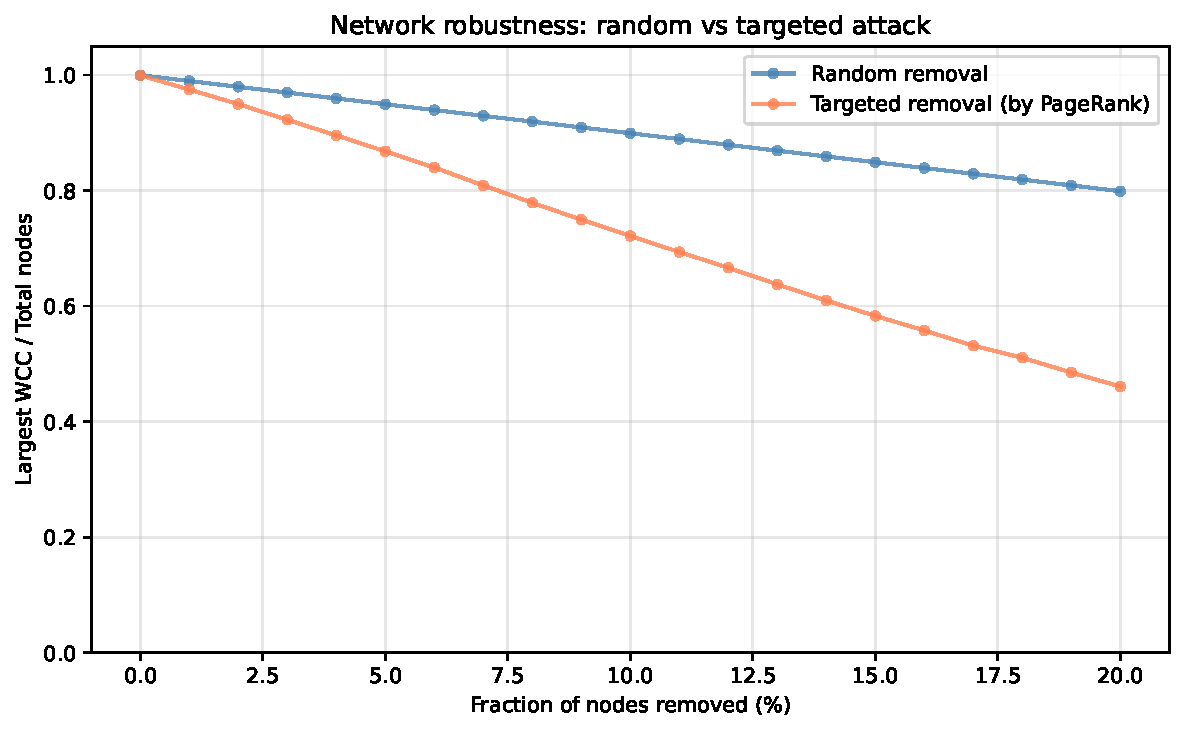
\includegraphics[width=0.85\textwidth]{analysis/thm_robustness_curve.pdf}
\caption{Robustness curves for $G_{\mathrm{thm}}$: fraction of nodes in the largest WCC as a function of the fraction removed, under random removal (indigo) and targeted removal by PageRank (gold).}
\label{fig:thm-robustness}
\end{figure}

Under random removal, the giant component shrinks almost linearly---removing $20\%$ of nodes leaves $80\%$ connected. Under targeted attack (removing the highest-PageRank nodes first), $20\%$ removal reduces connectivity to $46\%$---a $34$-percentage-point gap. This is the classic signature of a scale-free network~\cite{albert2000,barabasi1999}: resilient to random failure, vulnerable to targeted attack on hubs.

\begin{remark}
\label{rem:thm-robustness-redundancy}
The extreme resilience to single-node removal at the theorem level---no single declaration is a critical bridge---has a deeper explanation than mere edge density. It reflects the inherent \emph{logical redundancy} of mathematical proof. The same lemma is typically reachable through multiple independent proof paths: \decl{Eq.refl} can be circumvented via \texttt{rfl}, \decl{Eq.mpr}, or tactic-generated proof terms; a group-theoretic fact can be accessed through the group axioms or through the ring axioms that subsume them. This redundancy is not engineered (unlike the module-level redundancy of umbrella imports discussed in \S\ref{sec:transitive-reduction}); it is an intrinsic property of mathematical logic. The product carries its own structural insurance.
\end{remark}

\subsubsection{Namespace Level}
\label{sec:ns-robustness}

We assess the robustness of $G_{\mathrm{ns}}^{(2)}$ by progressively removing nodes and measuring the fraction of the original graph remaining in the largest weakly connected component (GCC). The original graph has $4$ weakly connected components, with the largest containing $10{,}094$ of $10{,}097$ nodes.

\begin{table}[ht]
\centering
\caption{Robustness of $G_{\mathrm{ns}}^{(2)}$: GCC fraction after random vs.\ targeted (PageRank-ordered) node removal.}
\label{tab:ns-robustness}
\begin{tabular}{rrrr}
\toprule
Removal \% & Random GCC & Targeted GCC & Gap \\
\midrule
$5\%$  & $0.950$ & $0.726$ & $0.223$ \\
$10\%$ & $0.899$ & $0.509$ & $0.391$ \\
$20\%$ & $0.798$ & $0.208$ & $0.590$ \\
$30\%$ & $0.688$ & $0.054$ & $0.634$ \\
$50\%$ & $0.477$ & $0.000$ & $0.477$ \\
\bottomrule
\end{tabular}
\end{table}

The pattern matches the classic scale-free vulnerability signature observed at both the module level (\S\ref{sec:robustness}) and the declaration level (\S\ref{sec:thm-robustness}): high resilience under random failure, extreme fragility under targeted attack (Table~\ref{tab:ns-robustness}). At $20\%$ targeted removal, the GCC collapses to $20.8\%$ of its original size---more severe than the declaration-level graph, where the same removal fraction leaves $46.1\%$ (\S\ref{sec:thm-robustness}). The namespace graph's greater fragility reflects the concentration of connectivity in the \ns{\_root\_} super-node and a small number of infrastructure namespaces (Remark~\ref{rem:root-artifact}); once these are removed, the remaining mathematical namespaces fragment into isolated clusters with no shared foundation.

%% ====================================================================
\subsection{Theorem vs.\ Lemma: Validating Human Importance Judgments}
\label{sec:thm-vs-lemma}

In Lean~4 source code, developers choose between \texttt{theorem} and \texttt{lemma} to declare propositions. While the kernel treats both identically---\texttt{lemma} is syntactic sugar for \texttt{theorem}---the choice carries cognitive significance: \texttt{theorem} typically marks a major result, while \texttt{lemma} signals an auxiliary stepping stone. Our extraction pipeline records both as kind \texttt{theorem}, erasing this distinction.

To recover it, we parsed the \module{Mathlib} source code, tracking \texttt{namespace} blocks to reconstruct fully qualified names, and cross-referenced with~$G_{\mathrm{thm}}$. Of the $251{,}642$ propositions in the graph, $175{,}567$ ($69.8\%$) were matched to a source declaration: $129{,}444$ marked \texttt{theorem} and $46{,}123$ marked \texttt{lemma}.

\begin{table}[ht]
\centering
\begin{tabular}{lccc}
\toprule
Metric & \texttt{theorem} & \texttt{lemma} & Ratio \\
\midrule
Mean in-degree        & $5.16$ & $3.52$ & $1.47\times$ \\
Zero-citation rate    & $37.2\%$ & $39.4\%$ & --- \\
Mean PageRank         & $7.52 \times 10^{-7}$ & $6.83 \times 10^{-7}$ & $1.10\times$ \\
\bottomrule
\end{tabular}
\caption{Structural comparison of declarations marked \texttt{theorem} vs.\ \texttt{lemma} in source code. All three metrics confirm that human importance judgments align with topological prominence.}
\label{tab:thm-vs-lemma}
\end{table}

All three metrics confirm that human importance judgments are validated by the logical structure: declarations that developers considered major results do occupy more prominent positions in the dependency network. The effect is moderate---a $1.47\times$ ratio in citation count, not an order-of-magnitude difference---suggesting that the theorem/lemma boundary is a noisy but genuine signal of structural importance.

\begin{remark}[Misjudged importance]
\label{rem:misjudged}
The alignment is imperfect. Among the notable outliers: \decl{funext} (function extensionality) is marked \texttt{lemma} in source code but has in-degree $15{,}574$, making it one of the most cited propositions in \module{Mathlib}. Conversely, $48{,}177$ declarations marked \texttt{theorem}---over a third of all matched theorems---have zero citations. The former represents underestimation of structural importance by the author; the latter represents overestimation, or more precisely, the distinction between importance as a mathematical result (worthy of the name ``theorem'') and importance as a dependency hub (actually reused by other proofs). In the language of our framework, the theorem/lemma distinction is a trace of the process---a record of the author's cognitive judgment at the time of writing---that the product partially but not fully corroborates.
\end{remark}
